\section{Components}
\label{sec:vanilla-components}

\begin{figure*}[t]
		\begin{minipage}[t]{0.5\linewidth}
		\begin{center}
                \subfigure[Regular \mhttp/TCP Stack.]{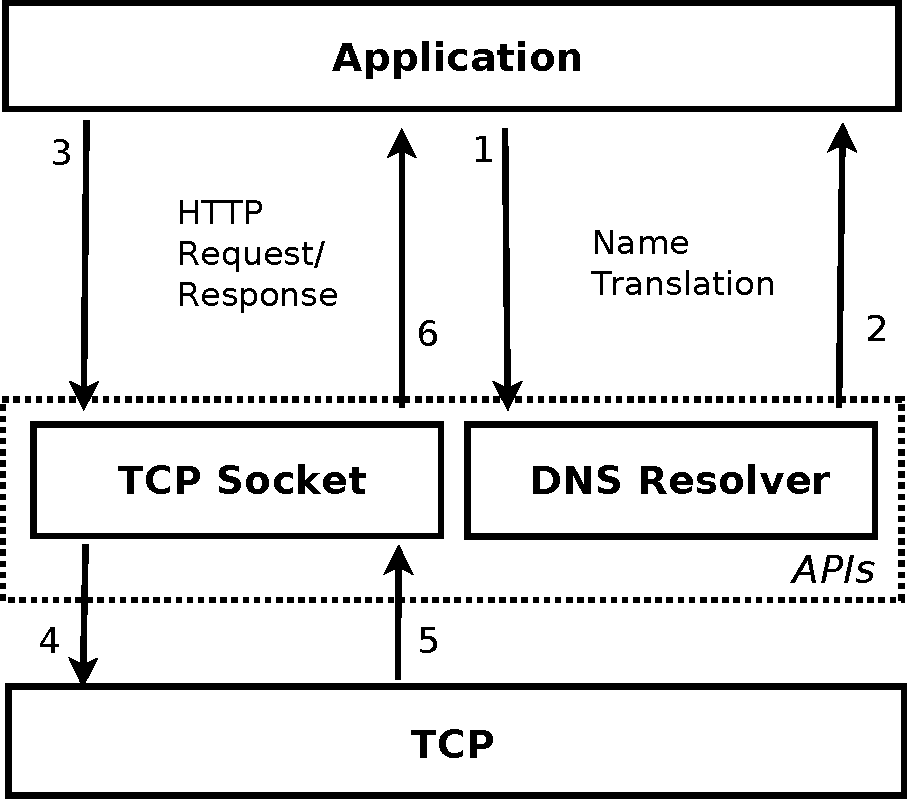
\includegraphics[width=\linewidth]{Figures/http-stack.pdf}}
        \end{center}
        \end{minipage}
~
        \begin{minipage}[t]{0.5\linewidth}
        \begin{center}
                \subfigure[\mhttp Stack on client.]{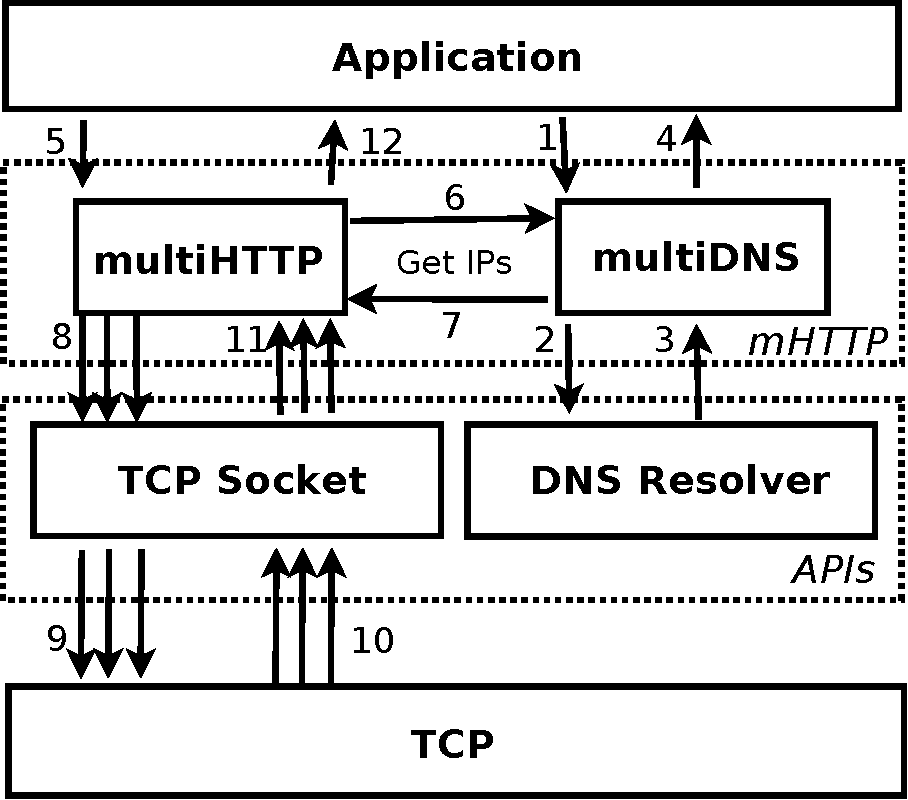
\includegraphics[width=\linewidth]{Figures/mhttp-stack.pdf}}
        \end{center}
        \end{minipage}
        \caption{\label{fig:stack-architecture} Architectural differences between regular HTTP (a) and \mhttp (b) (Figures inspired by previous studies~\cite{JKIM14-TUND}\cite{KIMSIG}\cite{KIM13-MHTTP}).}
  \vspace*{-0.3cm}
\end{figure*}

\mhttp~consists of two major components, \ie \term{multiHTTP} and \term{multiDNS}. 
\fref{fig:stack-architecture} illustrates the major differences between the common HTTP/TCP and the \mhttp~stack. 
We see that \term{multiHTTP} and \term{multiDNS} intercept calls from the application to the TCP layer, in order to manage multiple paths while staying completely transparent towards the application itself. 

\strong{multiHTTP} 
Handling chunked data delivery between the servers and the application is the major purpose of \term{multiHTTP}. 
Further, this module is responsible for the memory management, \ie a buffer in which partial data chunks can be stored even if they arrive out-of-order. 
Moreover, \term{multiHTTP} is responsible for manipulating HTTP request and response headers, \ie removing the response codes of subsequent responses and adding a chunk byte-range to the requests. 

\strong{multiDNS} 
\term{multiDNS} is used to retrieve and keep multiple IP addresses from different DNS servers in different ASes.
Usually an application uses only one server from a DNS query and discards the rest. 
\term{multiDNS} keeps the results of DNS queries from the application and stores all the retrieved IP addresses. 
Consequently, the main task for \term{multiDNS} is to discover and remember as many source servers as possible. 

